\documentclass[border=4pt]{standalone}

\usepackage{amsmath}
\usepackage{tikz}
\usepackage{mathdots}
\usepackage{yhmath}
\usepackage{cancel}
\usepackage{color}
\usepackage{siunitx}
\usepackage{array}
\usepackage{multirow}
\usepackage{amssymb}
\usepackage{gensymb}
\usepackage{tabularx}
\usepackage{booktabs}
\usetikzlibrary{fadings}
\usetikzlibrary{patterns}


\begin{document}
 


\tikzset{every picture/.style={line width=0.75pt}} %set default line width to 0.75pt        

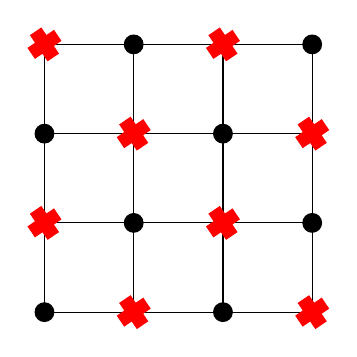
\begin{tikzpicture}[x=0.75pt,y=0.75pt,yscale=-1,xscale=1]
%uncomment if require: \path (0,300); %set diagram left start at 0, and has height of 300

%Shape: Grid [id:dp1464773156472241] 
\draw  [draw opacity=0] (160,50) -- (292.5,50) -- (292.5,182) -- (160,182) -- cycle ; \draw   (160,50) -- (160,182)(203,50) -- (203,182)(246,50) -- (246,182)(289,50) -- (289,182) ; \draw   (160,50) -- (292.5,50)(160,93) -- (292.5,93)(160,136) -- (292.5,136)(160,179) -- (292.5,179) ; \draw    ;
%Shape: Circle [id:dp6169476409350367] 
\draw  [color={rgb, 255:red, 0; green, 0; blue, 0 }  ,draw opacity=1 ][fill={rgb, 255:red, 0; green, 0; blue, 0 }  ,fill opacity=1 ] (155.5,93) .. controls (155.5,90.51) and (157.51,88.5) .. (160,88.5) .. controls (162.49,88.5) and (164.5,90.51) .. (164.5,93) .. controls (164.5,95.49) and (162.49,97.5) .. (160,97.5) .. controls (157.51,97.5) and (155.5,95.49) .. (155.5,93) -- cycle ;
%Shape: Circle [id:dp7028168097021623] 
\draw  [color={rgb, 255:red, 0; green, 0; blue, 0 }  ,draw opacity=1 ][fill={rgb, 255:red, 0; green, 0; blue, 0 }  ,fill opacity=1 ] (198.5,50) .. controls (198.5,47.51) and (200.51,45.5) .. (203,45.5) .. controls (205.49,45.5) and (207.5,47.51) .. (207.5,50) .. controls (207.5,52.49) and (205.49,54.5) .. (203,54.5) .. controls (200.51,54.5) and (198.5,52.49) .. (198.5,50) -- cycle ;
%Shape: Circle [id:dp752605133583879] 
\draw  [color={rgb, 255:red, 0; green, 0; blue, 0 }  ,draw opacity=1 ][fill={rgb, 255:red, 0; green, 0; blue, 0 }  ,fill opacity=1 ] (198.5,136) .. controls (198.5,133.51) and (200.51,131.5) .. (203,131.5) .. controls (205.49,131.5) and (207.5,133.51) .. (207.5,136) .. controls (207.5,138.49) and (205.49,140.5) .. (203,140.5) .. controls (200.51,140.5) and (198.5,138.49) .. (198.5,136) -- cycle ;
%Shape: Circle [id:dp010139644248294166] 
\draw  [color={rgb, 255:red, 0; green, 0; blue, 0 }  ,draw opacity=1 ][fill={rgb, 255:red, 0; green, 0; blue, 0 }  ,fill opacity=1 ] (241.5,93) .. controls (241.5,90.51) and (243.51,88.5) .. (246,88.5) .. controls (248.49,88.5) and (250.5,90.51) .. (250.5,93) .. controls (250.5,95.49) and (248.49,97.5) .. (246,97.5) .. controls (243.51,97.5) and (241.5,95.49) .. (241.5,93) -- cycle ;
%Shape: Circle [id:dp40937764599964366] 
\draw  [color={rgb, 255:red, 0; green, 0; blue, 0 }  ,draw opacity=1 ][fill={rgb, 255:red, 0; green, 0; blue, 0 }  ,fill opacity=1 ] (155.5,179) .. controls (155.5,176.51) and (157.51,174.5) .. (160,174.5) .. controls (162.49,174.5) and (164.5,176.51) .. (164.5,179) .. controls (164.5,181.49) and (162.49,183.5) .. (160,183.5) .. controls (157.51,183.5) and (155.5,181.49) .. (155.5,179) -- cycle ;
%Shape: Circle [id:dp9047801372360353] 
\draw  [color={rgb, 255:red, 0; green, 0; blue, 0 }  ,draw opacity=1 ][fill={rgb, 255:red, 0; green, 0; blue, 0 }  ,fill opacity=1 ] (241.5,179) .. controls (241.5,176.51) and (243.51,174.5) .. (246,174.5) .. controls (248.49,174.5) and (250.5,176.51) .. (250.5,179) .. controls (250.5,181.49) and (248.49,183.5) .. (246,183.5) .. controls (243.51,183.5) and (241.5,181.49) .. (241.5,179) -- cycle ;
%Shape: Circle [id:dp1217522971084728] 
\draw  [color={rgb, 255:red, 0; green, 0; blue, 0 }  ,draw opacity=1 ][fill={rgb, 255:red, 0; green, 0; blue, 0 }  ,fill opacity=1 ] (284.5,136) .. controls (284.5,133.51) and (286.51,131.5) .. (289,131.5) .. controls (291.49,131.5) and (293.5,133.51) .. (293.5,136) .. controls (293.5,138.49) and (291.49,140.5) .. (289,140.5) .. controls (286.51,140.5) and (284.5,138.49) .. (284.5,136) -- cycle ;
%Shape: Circle [id:dp5239361962483693] 
\draw  [color={rgb, 255:red, 0; green, 0; blue, 0 }  ,draw opacity=1 ][fill={rgb, 255:red, 0; green, 0; blue, 0 }  ,fill opacity=1 ] (284.5,50) .. controls (284.5,47.51) and (286.51,45.5) .. (289,45.5) .. controls (291.49,45.5) and (293.5,47.51) .. (293.5,50) .. controls (293.5,52.49) and (291.49,54.5) .. (289,54.5) .. controls (286.51,54.5) and (284.5,52.49) .. (284.5,50) -- cycle ;
%Shape: Cross [id:dp6145616981205815] 
\draw  [color={rgb, 255:red, 255; green, 0; blue, 0 }  ,draw opacity=1 ][fill={rgb, 255:red, 255; green, 0; blue, 0 }  ,fill opacity=1 ] (164.53,43.38) -- (167.82,48.24) -- (164.18,50.71) -- (166.65,54.35) -- (161.58,57.79) -- (159.11,54.15) -- (155.47,56.62) -- (152.18,51.76) -- (155.82,49.29) -- (153.35,45.65) -- (158.42,42.21) -- (160.89,45.85) -- cycle ;
%Shape: Cross [id:dp9589423652124174] 
\draw  [color={rgb, 255:red, 255; green, 0; blue, 0 }  ,draw opacity=1 ][fill={rgb, 255:red, 255; green, 0; blue, 0 }  ,fill opacity=1 ] (207.53,86.38) -- (210.82,91.24) -- (207.18,93.71) -- (209.65,97.35) -- (204.58,100.79) -- (202.11,97.15) -- (198.47,99.62) -- (195.18,94.76) -- (198.82,92.29) -- (196.35,88.65) -- (201.42,85.21) -- (203.89,88.85) -- cycle ;
%Shape: Cross [id:dp10981573516059617] 
\draw  [color={rgb, 255:red, 255; green, 0; blue, 0 }  ,draw opacity=1 ][fill={rgb, 255:red, 255; green, 0; blue, 0 }  ,fill opacity=1 ] (164.53,129.38) -- (167.82,134.24) -- (164.18,136.71) -- (166.65,140.35) -- (161.58,143.79) -- (159.11,140.15) -- (155.47,142.62) -- (152.18,137.76) -- (155.82,135.29) -- (153.35,131.65) -- (158.42,128.21) -- (160.89,131.85) -- cycle ;
%Shape: Cross [id:dp6065846693378949] 
\draw  [color={rgb, 255:red, 255; green, 0; blue, 0 }  ,draw opacity=1 ][fill={rgb, 255:red, 255; green, 0; blue, 0 }  ,fill opacity=1 ] (250.53,43.38) -- (253.82,48.24) -- (250.18,50.71) -- (252.65,54.35) -- (247.58,57.79) -- (245.11,54.15) -- (241.47,56.62) -- (238.18,51.76) -- (241.82,49.29) -- (239.35,45.65) -- (244.42,42.21) -- (246.89,45.85) -- cycle ;
%Shape: Cross [id:dp8827376073467343] 
\draw  [color={rgb, 255:red, 255; green, 0; blue, 0 }  ,draw opacity=1 ][fill={rgb, 255:red, 255; green, 0; blue, 0 }  ,fill opacity=1 ] (207.53,172.38) -- (210.82,177.24) -- (207.18,179.71) -- (209.65,183.35) -- (204.58,186.79) -- (202.11,183.15) -- (198.47,185.62) -- (195.18,180.76) -- (198.82,178.29) -- (196.35,174.65) -- (201.42,171.21) -- (203.89,174.85) -- cycle ;
%Shape: Cross [id:dp2687178397547334] 
\draw  [color={rgb, 255:red, 255; green, 0; blue, 0 }  ,draw opacity=1 ][fill={rgb, 255:red, 255; green, 0; blue, 0 }  ,fill opacity=1 ] (250.53,129.38) -- (253.82,134.24) -- (250.18,136.71) -- (252.65,140.35) -- (247.58,143.79) -- (245.11,140.15) -- (241.47,142.62) -- (238.18,137.76) -- (241.82,135.29) -- (239.35,131.65) -- (244.42,128.21) -- (246.89,131.85) -- cycle ;
%Shape: Cross [id:dp33987705601992957] 
\draw  [color={rgb, 255:red, 255; green, 0; blue, 0 }  ,draw opacity=1 ][fill={rgb, 255:red, 255; green, 0; blue, 0 }  ,fill opacity=1 ] (293.53,86.38) -- (296.82,91.24) -- (293.18,93.71) -- (295.65,97.35) -- (290.58,100.79) -- (288.11,97.15) -- (284.47,99.62) -- (281.18,94.76) -- (284.82,92.29) -- (282.35,88.65) -- (287.42,85.21) -- (289.89,88.85) -- cycle ;
%Shape: Cross [id:dp7388958172952218] 
\draw  [color={rgb, 255:red, 255; green, 0; blue, 0 }  ,draw opacity=1 ][fill={rgb, 255:red, 255; green, 0; blue, 0 }  ,fill opacity=1 ] (293.53,172.38) -- (296.82,177.24) -- (293.18,179.71) -- (295.65,183.35) -- (290.58,186.79) -- (288.11,183.15) -- (284.47,185.62) -- (281.18,180.76) -- (284.82,178.29) -- (282.35,174.65) -- (287.42,171.21) -- (289.89,174.85) -- cycle ;




\end{tikzpicture}
\end{document}
